%2multibyte Version: 5.50.0.2953 CodePage: 1252

\documentclass[bigger]{beamer}
%%%%%%%%%%%%%%%%%%%%%%%%%%%%%%%%%%%%%%%%%%%%%%%%%%%%%%%%%%%%%%%%%%%%%%%%%%%%%%%%%%%%%%%%%%%%%%%%%%%%%%%%%%%%%%%%%%%%%%%%%%%%%%%%%%%%%%%%%%%%%%%%%%%%%%%%%%%%%%%%%%%%%%%%%%%%%%%%%%%%%%%%%%%%%%%%%%%%%%%%%%%%%%%%%%%%%%%%%%%%%%%%%%%%%%%%%%%%%%%%%%%%%%%%%%%%
\usepackage{amsfonts}
\usepackage{amsmath}
\usepackage{mathpazo}

\usepackage{graphicx}
\usepackage{pdfpages}
\usepackage{hyperref}
\usepackage{multimedia}



\hypersetup{
    colorlinks=true,
    linkcolor=blue,
    filecolor=magenta,      
    urlcolor=cyan,
}
 
\urlstyle{same}
% 
% \setcounter{MaxMatrixCols}{10}
%TCIDATA{OutputFilter=LATEX.DLL}
%TCIDATA{Version=5.50.0.2953}
%TCIDATA{Codepage=1252}
%TCIDATA{<META NAME="SaveForMode" CONTENT="1">}
%TCIDATA{BibliographyScheme=Manual}
%TCIDATA{Created=Monday, October 27, 2008 15:56:24}
%TCIDATA{LastRevised=Monday, March 20, 2017 13:11:45}
%TCIDATA{<META NAME="GraphicsSave" CONTENT="32">}
%TCIDATA{<META NAME="DocumentShell" CONTENT="Other Documents\SW\Slides - Beamer">}
%TCIDATA{CSTFile=beamer.cst}

% \newenvironment{stepenumerate}{\begin{enumerate}[<+->]}{\end{enumerate}}
% \newenvironment{stepitemize}{\begin{itemize}[<+->]}{\end{itemize} }
% \newenvironment{stepenumeratewithalert}{\begin{enumerate}[<+-| alert@+>]}{\end{enumerate}}
% \newenvironment{stepitemizewithalert}{\begin{itemize}[<+-| alert@+>]}{\end{itemize} }

%\let\TEXTsymbol\ensuremath 
%\newcommand\tsum{\textstyle\sum\nolimits}

\usetheme{Madrid}
\usecolortheme{beaver}
\usefonttheme{professionalfonts}
\input{tcilatex}
\setbeamertemplate{navigation symbols}{}

\begin{document}

\title[47-809: Linear equations]{Linear equations and iterative methods}
\subtitle{Judd Chapter 3}
\author[David Childers]{David Childers (thanks to Y. Kryukov, K. Judd, and U. Doraszelski)}
\institute[CMU]{CMU, Tepper School of Business}
\date[Mar-15]{ March 15, 2023}
\maketitle

\section{Linear equations and Iterative methods}

\begin{frame}
\frametitle{Numerical Linear Algebra}

\begin{itemize}

\item Linear algebra is basic building block of numerical mathematics
\item Algorithms extremely well developed: every language has low and medium level library implementing efficient algorithms
\begin{itemize}
\item \emph{BLAS}: Basic Linear Algebra Subprograms to implement basics, eg OpenBLAS/MKL 
\item Mid-level: LAPACK almost universal for standard implementations of applied algorithms
\item High-level: Julia \href{https://docs.julialang.org/en/v1/stdlib/LinearAlgebra/}{LinearAlgebra}, Python \href{https://docs.scipy.org/doc/scipy/reference/linalg.html}{scipy}/\href{https://numpy.org/devdocs/reference/routines.linalg.html}{numpy} \texttt{linalg} 
\item Specialized libraries: (eg for deep learning) reimplement to take advantage of hardware (GPU, etc) or extra structure
\end{itemize}

\item You should understand building blocks of these algorithms: speed, robustness, accuracy in different situations
\item Core problems 
  \begin{itemize}
     \item \texttt{A*B} / \texttt{A @ B}, \texttt{A\textbackslash b}, \texttt{eig(A)} / \texttt{eigen(A)}, etc. 
    \item Many implementations each, with different tradeoffs
  \end{itemize}

\end{itemize}


\end{frame}

\begin{frame}
\frametitle{Warmup: Matrix Muliplication}
\begin{itemize}
\item Let A, B be $n\times n$ matrices
\item Naive algorithm follows from definition of $A*B$
\begin{equation*}
\left[A*B\right]_{ij}=\sum_{k=1}^{n}A_{ik}B_{kj}
\end{equation*}
\item Takes $n$ multiplications and additions for each of $n^2$ entries 
  \begin{itemize}
    \item $O(2n^3)$ operations total
  \end{itemize}
\item Coppersmith-Winograd algorithm is $\approx$ $O(n^{2.37})$
  \begin{itemize}
    \item But constant large: only use if n huge
  \end{itemize}
\item Default implementations have cost in between (e.g. $O(n^{2.81})$)
\item Matrix-vector multiply $A*b$, $b$ $n\times 1$ is $O(2n^2)$ by same logic

\end{itemize}


\end{frame}

\begin{frame}%
\frametitle{Exploiting Structure}

\begin{itemize}

\item Many matrices arising in practice have additional structure

\begin{itemize}
\item Symmetric, Diagonal, Toeplitz, triangular, sparse, low rank, etc
\end{itemize}

\item Sparse matrices have $m<<n^2$ nonzero entries
\item Toeplitz \& circulant matrices occur under invariances
\item Fast algorithms exist which depend on structure: e.g.
  \begin{itemize}
  \item Diagonal (or tridiagonal) matrix multiplication is $O(n)$
  \item Circulant matrix-vector multiplication is $O(n\log (n))$: FFT
  \item Will use this for interpolation, etc
  \end{itemize}
\item Some algorithms work for all matrices, faster when structured
\item Others need explicit info about structure: use \emph{types} to represent
\item See \texttt{scipy.linalg} or \href{https://github.com/JuliaLinearAlgebra}{JuliaLinearAlgebra} library families

\end{itemize}

\end{frame}

\begin{frame}%
%EndExpansion

\frametitle{The Plan: systems of linear equations}

\begin{itemize}
\item Direct methods -- reliable but slow

\begin{itemize}
\item Back substitution

\item LU decomposition

\item QR and Cholesky decompositions
\end{itemize}

\item Measuring precision: Eigenvalues and condition numbers

\item Iterative methods:

\begin{itemize}
\item Classic version -- Gauss-Jacobi

\item An improvement -- Gauss-Seidel

\item Convergence, dampening and acceleration

\item Alternatives
\end{itemize}

\item Technical improvements: parallelization, randomization, sparsity

\item Application: Eigenvectors and Markov chains

\end{itemize}


\end{frame}%


\begin{frame}%
%EndExpansion
\frametitle{Systems of linear equations}

\begin{equation*}
Ax=b,
\end{equation*}%
where $A$ is an $n\times n$ matrix, $x$ and $b$ are $n\times 1$
vectors\bigskip

\begin{itemize}
\item Some simple economic problems are linear:

\begin{itemize}
\item General Equilibrium with linear supply and demand

\item OLS estimator: $\left( X^{\prime }X\right) \hat{\beta}=X^{\prime }Y$
\end{itemize}

\item Used as a building block in other methods

\begin{itemize}
\item Newton's method for nonlinear equations or optimization

\item Polynomial or spline coefficients in approximation

\item Value function in policy iteration

\item Ergodic (stable) distribution of Markov Chain
\end{itemize}

\item Simple example used to illustrate iterative methods
\end{itemize}

%TCIMACRO{\TeXButton{EndFrame}{\end{frame}}}%
%BeginExpansion
\end{frame}%
%EndExpansion
%TCIMACRO{\TeXButton{BeginFrame}{\begin{frame}}}%
%BeginExpansion
\begin{frame}%
%EndExpansion
\frametitle{Back-substitution}

Suppose $A$ is lower triangular, i.e, 
\begin{equation*}
A=\left( 
\begin{array}{cccc}
a_{11} & 0 & \cdots & 0 \\ 
a_{21} & a_{22} & \cdots & 0 \\ 
\vdots & \vdots & \ddots & \vdots \\ 
a_{n1} & a_{n2} & \cdots & a_{nn}%
\end{array}%
\right) .
\end{equation*}%
Then we can easily solve it: 
\begin{eqnarray*}
x_{1} &=&\frac{b_{1}}{a_{11}}, \\
x_{k} &=&\frac{b_{k}-\sum_{j=1}^{k-1}a_{kj}x_{j}}{a_{kk}},\quad k=2,3,\ldots
,n.
\end{eqnarray*}


\end{frame}%


\begin{frame}

\frametitle{LU decomposition}

\begin{itemize}
\item Find $L$ and $U$ such that: 
\begin{equation*}
A=LU
\end{equation*}

\begin{itemize}
\item $L$ is \textbf{L}ower triangular

\item $U$ is \textbf{U}pper triangular

\item Matlab/Julia (LinearAlgebra)/Scipy: \texttt{lu(A)}
\end{itemize}

\item Solving system of equations $Ax=b\Leftrightarrow L[Ux]=b$:

\begin{itemize}
\item Find $L$ and $U$

\item Solve $Lz=b$ for $z$ by back-substitution

\item Solve $Ux=z$ for $x$ by back-substitution

\item Matlab/Julia: \texttt{x = A\TEXTsymbol{\backslash}b} \ \ (backslash or "left
division") Numpy/scipy \texttt{solve(A,b)}
\end{itemize}
\end{itemize}


\end{frame}%


\begin{frame}%


\frametitle{Other Decompositions}

\begin{itemize}
\item \textbf{QR decomposition}: $A=QR$. 

\begin{itemize}
\item $Q$ is orthogonal ($Q^{\prime }Q$ is an identity matrix),

\item $R$ is upper triangular.
\item Matlab/Julia/Numpy/Scipy: \texttt{qr(A)}
\end{itemize}

\item Solution: $Ax=b\Leftrightarrow Q^{\prime }QRx=Q^{\prime }b$,

\begin{itemize}
\item $Q^{\prime }QR$ is upper triangular $\Rightarrow $ solve for $x$ by
back-substitution

\item One back-substitution, but decomposition takes longer\bigskip
\end{itemize}

\item \textbf{Cholesky decomposition} ("square root" of $A$)

\begin{itemize}
\item Exists if $A$ is symmetric and positive definite

\item $A=CC^{\prime }$, $C$ is lower triangular ($\Rightarrow $ $C^{\prime }$
-- upper).

\item Matlab: \texttt{chol(A)} Julia/Numpy/Scipy: \texttt{cholesky(A)}
\end{itemize}
\end{itemize}


\end{frame}%

\begin{frame}%

\frametitle{A bit of theory: matrix analysis}

\begin{itemize}
\item $\lambda \in \mathbb{C}$ is an \textbf{eigenvalue} of $n\times n$
matrix $A$ iff:

\begin{itemize}
\item there is an eigenvector $v\in \mathbb{C}^{n}$, $v\neq 0$, ...

\item ... such that $Av=\lambda v$, and $\det (A-\lambda I)=0$.
\end{itemize}

\item \textbf{Spectrum} $\sigma (A)$ = set of all $n$ eigenvalues

\begin{itemize}
\item Matlab/Numpy/Scipy: \texttt{eig(A)} Julia: \texttt{eigvals(A)}
\end{itemize}

\item \textbf{Spectral radius} $\rho (A):=\max \left\vert \sigma
(A)\right\vert $

\item \textbf{Norm}: $||A||=\max_{x\neq 0}\frac{||Ax||}{||x||}%
=\max_{||x||=1}||Ax||$ \texttt{= norm(A) } / \texttt{opnorm(A) }

\item \textbf{Condition number}: $cond(A)=||A||\cdot ||A^{-1}||$ \texttt{=
cond(A)}

\begin{itemize}
\item If $A$ is singular, then the condition number is +$\infty $.

\item If $A$ is near-singular, condition number is high (\TEXTsymbol{>}10$%
^{10}$)
\end{itemize}

\item \textbf{Spectral condition number}: $cond_{\ast }(A)=\rho (A)/\min
\left\vert \sigma (A)\right\vert $

\begin{itemize}
\item $cond(A)\geq cond_{\ast }(A)$

\item They tend to have same order of magnitude ($m$ in $10^{m}$)
\end{itemize}
\end{itemize}


\end{frame}%

\begin{frame}%

\frametitle{Bounding the errors}

\begin{itemize}
\item Perturb the system by $r$: $A\tilde{x}=b+r$ \ (e.g. due to rounding)%
\newline
$\Longrightarrow $\ Error $e=\tilde{x}-x$.

\item Elasticity of solution w.r.t. error:%
\begin{equation*}
\frac{1}{cond(A)}\leq \frac{||e||/||x||}{||r||/||b||}\leq cond(A).
\end{equation*}

\item Rule of thumb: each order of magnitude in condition number loses one
decimal digit of accuracy from $x$

\item Since we only care about orders of magnitude, \newline
we can use $cond_{\ast }(A)$ instead -- it is a lot faster to compute.

\item $\Rightarrow $ Pre-conditioning: pick $D$ so $DA$ is well-conditioned,
solve 
\begin{equation*}
\left( DA\right) x=\left( Db\right)
\end{equation*}
\end{itemize}

%TCIMACRO{\TeXButton{EndFrame}{\end{frame}}}%
%BeginExpansion
\end{frame}%


\begin{frame}%

\frametitle{Speed of computation}

\begin{itemize}
\item LU decomposition:

\begin{itemize}
\item Decomposition: $n^{3}/3$ multiplications and divisions

\item Backward substitution: $n^{2}$ multiplications and divisions
\end{itemize}

\item QR decomposition -- also $Kn^{3}$ operations\bigskip

\item Cramer's rule (determinants) = $n!$ operations = very slow

\begin{itemize}
\item It is useful in theory work, as an expression for solution\bigskip
\end{itemize}

\item We can often improve speed \newline
at cost of a bit of precision

\begin{itemize}
\item $\Longrightarrow $ Iterative methods
\end{itemize}
\end{itemize}

%TCIMACRO{\TeXButton{EndFrame}{\end{frame}}}%
%BeginExpansion
\end{frame}%
%EndExpansion
%TCIMACRO{\TeXButton{BeginFrame}{\begin{frame}}}%
%BeginExpansion
\begin{frame}%
%EndExpansion
\frametitle{Gauss-Jacobi iterations}

\begin{itemize}
\item Idea: solve $i$-th equation for $x_{i}$ alone:%
\begin{gather*}
\tsum\nolimits_{j=1}^{n}a_{ij}x_{j}=b_{i} \\
\Rightarrow x_{i}=\frac{1}{a_{ii}}\left\{ b_{i}-\tsum\nolimits_{j\neq
i}^{{}}a_{ij}x_{j}\right\}
\end{gather*}

\item Use it to iterate: have guess $x^{k}$, compute $x^{k+1}$ as:%
\begin{equation*}
x_{i}^{k+1}=\frac{1}{a_{ii}}\left\{ b_{i}-\tsum\nolimits_{j\neq
i}^{n}a_{ij}x_{j}^{k}\right\} ,\quad i=1,\ldots ,n
\end{equation*}

\item Need a starting guess $x^{0}$.

\item Need a stopping rule, e.g.:%
\begin{equation*}
\frac{\left\Vert x^{k+1}-x^{k}\right\Vert }{\left\Vert x^{k}\right\Vert +1}%
<\delta
\end{equation*}
\end{itemize}


\end{frame}%


\begin{frame}%
%EndExpansion
\frametitle{Gauss-Seidel}

\begin{itemize}
\item Gauss-Jacobi computes the last element ($x_{n}^{k+1}$) as:%
\begin{equation*}
x_{n}^{k+1}=\frac{1}{a_{ii}}\left\{
b_{i}-\tsum\nolimits_{j=1}^{n-1}a_{ij}x_{j}^{k}\right\}
\end{equation*}

\begin{itemize}
\item If we update elements in natural order ($1,...,n$)\newline
we already have $x_{1}^{k+1},...,x_{n-1}^{k+1}$ computed.

\item It would speed things up to use them rather than $x^{k}$
\end{itemize}

\item Gauss-Seidel does the same for every element $x_{i}^{k+1}$:%
\begin{equation*}
x_{i}^{k+1}=\frac{1}{a_{ii}}\left\{
b_{i}-\tsum\nolimits_{j=1}^{i-1}a_{ij}x_{j}^{k+1}-\tsum%
\nolimits_{j=i+1}^{n}a_{ij}x_{j}^{k}\right\}
\end{equation*}

\item See Figure 3.2 in the textbook for an illustration.
\end{itemize}

%TCIMACRO{\TeXButton{EndFrame}{\end{frame}}}%
%BeginExpansion
\end{frame}%


\begin{frame}%

\frametitle{Figure 3.2}

\scalebox{0.55}{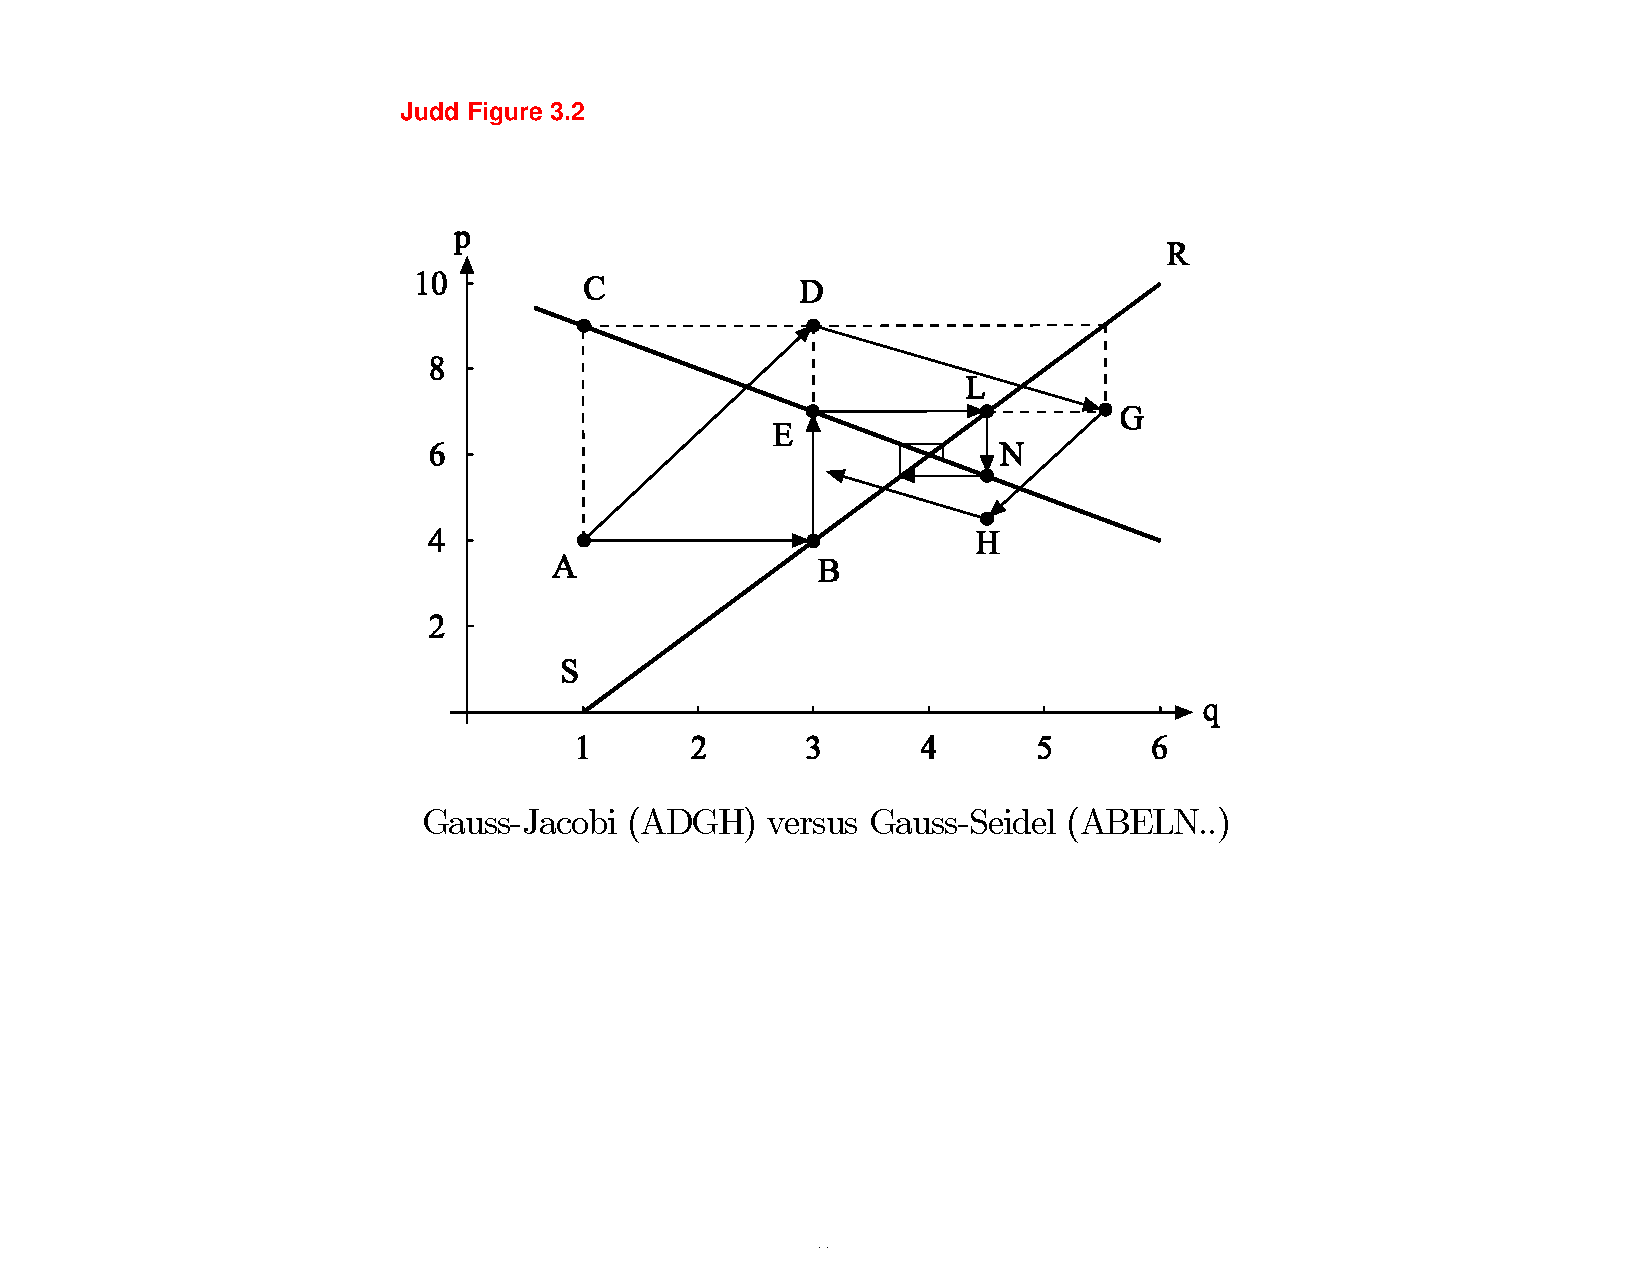
\includegraphics[page=1]{Chap3Linear_figures.pdf}}




\end{frame}%



\begin{frame}%
%EndExpansion
\frametitle{Convergence and operator splitting}

\begin{itemize}
\item Operator splitting: $A=(N-P)$%
\begin{eqnarray*}
Nx &=&b+Px \\
x^{k+1} &=&N^{-1}(b+Px^{k})
\end{eqnarray*}

\item $N$ is selected so it is easy to invert:

\begin{itemize}
\item GJ: $N$ is the diagonal of $A$

\item GS (using natural order): $N$ is the lower triangle of $A$
\end{itemize}

\item GJ/GS are linearly convergent at rate $\rho (N^{-1}P)$

\item Condition for convergence: $\rho (N^{-1}P)<1$

\begin{itemize}
\item $\iff $ all eigenvalues are inside the unit circle

\item $\Leftarrow $ Matrix $A$ diagonally dominant: $\left\vert
a_{ii}\right\vert >\sum_{j\neq i}\left\vert a_{ij}\right\vert $

\item 1-dimensional interpretation: slope less than 1
\end{itemize}
\end{itemize}

%TCIMACRO{\TeXButton{EndFrame}{\end{frame}}}%
%BeginExpansion
\end{frame}%



\begin{frame}%

\frametitle{Precision under linear convergence}

\begin{itemize}
\item Linear convergence (plus some conditions) imply: \newline
$\left\Vert x^{k+1}-x^{k}\right\Vert \leq \beta \left\Vert
x^{k}-x^{k-1}\right\Vert $

\begin{itemize}
\item where $\beta $ is the linear convergence rate
\end{itemize}

\item It follows that $\left\Vert x^{k}-x^{\ast }\right\Vert \leq \left\Vert
x^{k+1}-x^{k}\right\Vert /\left( 1-\beta \right) $

\begin{itemize}
\item To prove, use triangle inequality
\end{itemize}

\item So, if we want to ensure $\left\Vert x^{k}-x^{\ast }\right\Vert
<\delta $, stop when%
\begin{equation*}
\left\Vert x^{k+1}-x^{k}\right\Vert \leq \delta \left( 1-\beta \right)
\end{equation*}

\item Since we do not know $\beta $, we can estimate: $\hat{\beta}%
=\max_{\kappa =1,...,k}\left\{ \left\Vert x^{\kappa }-x^{\kappa
-1}\right\Vert /\left\Vert x^{\kappa -1}-x^{\kappa -2}\right\Vert \right\} $

\item Of course, this approach is valid only if there is convergence
\end{itemize}

\end{frame}


\begin{frame}
\frametitle{Guarantees for iterative methods}

 \begin{itemize}

\item Gerschgorin circle theorem:
\begin{itemize}
  \item Let $A$ have eigenvalues $\{\lambda_s\}_{s=1}^{n}$, $R_i=\sum_{j\neq i}\left\vert a_{ij}\right\vert$
  \item Then $\lambda_s\in \cup_{i=1}^{n} B(a_{ii},R_i)$ $\forall s$
\end{itemize}  

\item Corollary: If $A$ is diagonally dominant with $\beta=\sup\{\left\vert x \right\vert:\ x\in\cup_{i=1}^{n} B(a_{ii}^{-1},R_i)\}<1$, then Gauss-Jacobi converges to within error $\delta$ in $O(n^2\log(\frac{1}{\delta}))$ operations

\item Informal proof:
\begin{itemize}
  \item Each iteration is a diagonal matrix multiply, which is $O(n^2)$
  \item Gerschgorin$\implies\rho(N^{-1}P)\leq\beta<1,\implies$ linear convergence
\end{itemize}

\item Compare $O(n^3)$ for direct methods
\begin{itemize}
\item Substantial improvement even for machine precision error
\end{itemize}

\item For G-S, can show $A$ diagonal dominant OR symmetric positive definite $\implies\rho(N^{-1}P)<1$
\begin{itemize}
\item Occurs in least squares problems, many 2nd order PDEs
\end{itemize}

\item These structures are sufficient, not necessary


\end{itemize}

\end{frame}


\begin{frame}%
%EndExpansion
\frametitle{Dampening: a tweak to iterations}

\begin{itemize}
\item Gauss-Jacobi algorithm takes steps $\Delta x$ at each iteration:

\begin{itemize}
\item Each iteration computes $x^{k+1}=N^{-1}Px^{k}+N^{-1}b=Gx^{k}+d$

\item Step is $\Delta x^{k+1}=x^{k+1}-x^{k}=Gx^{k}+d-x^{k}$
\end{itemize}

\item We can choose to scale $\Delta x^{k+1}$ by $\omega $:%
\begin{equation*}
x^{k+1}=\omega \lbrack Gx^{k}+d]+(1-\omega )x^{k}
\end{equation*}

\item $\omega <1$: Stabilization / dampening:

\begin{itemize}
\item can create or speed up convergence

\item avoids exploding or going in circles around the solution

\item See Figure 3.4 in the texbook for an illustration.
\end{itemize}

\item $\omega >1$: Extrapolation -- speeds up convergence (Fig. 3.5)
\end{itemize}


\end{frame}%

\begin{frame}%

\frametitle{Figure 3.4}

\scalebox{0.40}{\includegraphics[page=2]{Chap3Linear_figures.pdf}}


\end{frame}%

\begin{frame}%

\frametitle{Figure 3.5}

\scalebox{0.40}{\includegraphics[page=3]{Chap3Linear_figures.pdf}}


\end{frame}%

\begin{frame}%

\frametitle{Dampening and convergence}

\begin{itemize}
\item If all eigenvalues $\sigma (G)$ are real, optimal dampening is%
\begin{equation*}
\omega ^{\ast }=\frac{2}{2-\max \left\vert \sigma (G)\right\vert -\min
\left\vert \sigma (G)\right\vert }
\end{equation*}

\item Weyl's inequality states that $\sigma \{\omega G+(1-\omega )I\}\leq\omega \sigma
(G)+(1-\omega )$

\begin{itemize}
\item Dampening shifts (potentially complex) eigenvalues towards 1

\item If $\max \func{real}\{\sigma (G)\}<1$, dampening can restore stability 
\newline
and improve convergence speed.

\item If $\max \func{real}\{\sigma (G)\}>1$, dampening cannot restore
stability.
\end{itemize}

\item Can combine dampening with G-S (Successive overrelaxation)

\begin{itemize}
\item Potentially even bigger gains
\end{itemize}
\end{itemize}


\end{frame}%
%EndExpansion
%TCIMACRO{\TeXButton{BeginFrame}{\begin{frame}}}%
%BeginExpansion
\begin{frame}%
%EndExpansion

\frametitle{Preview: nonlinear GS/GJ methods}

\begin{itemize}
\item We can (and will) use iterative methods \newline
for nonlinear fixed-point problems: $x=F(x)$

\item For $\sigma (G)$ and $\rho (G)$, $G$ is the Jacobian of $F$

\item Convergence properties are local, \newline
and we can have more than one solution

\item Dampening works exactly as described

\item In general, convergence does not necessarily imply a solution

\item For linear problem, we can \textbf{verify} solution by computing 
\begin{equation*}
\left\Vert Ax-b\right\Vert
\end{equation*}

\begin{itemize}
\item For nonlinear fixed point problem, no general test
\end{itemize}
\end{itemize}


\end{frame}%

\begin{frame}%

\frametitle{Alternatives: Krylov subspace methods}

\begin{itemize}

\item eg \emph{Conjugate Gradient} for pos. def. $A$: \emph{GMRES} for general $A$

\item Combines strengths of iterative and direct methods

\item "Exact" convergence in $n$ iterations by building solution from sequence of linearly independent vectors
\begin{itemize}
\item Floating point error accumulates, worse than direct methods 
\item Practical implementations require fixes: see Golub \& van Loan
\end{itemize}

\item Each iteration uses $A$ only in small $\#$ of matrix-vector multiplies

\item No real gain over direct methods if no structure: $n\times O(n^2)$ ops
\item Substantial gain in speed if 
\begin{enumerate}
\item Matrix-vector multiplies are fast: sparse, structured, etc
\item $b$ (nearly) restricted to low-d subspace, or initial guess good
\item Preconditioning can help ensure this
\begin{itemize}
\item Cut off at small $\#$ of iterations for small loss in accuracy
\end{itemize}
\end{enumerate}






\end{itemize}


\end{frame}%


\begin{frame}%
%EndExpansion
\frametitle{Parallelization}

\begin{itemize}
\item GJ\ with single CPU computes $x_{i}^{k+1}$'s one after another

\item If we have many CPUs, we can parallelize:

\begin{itemize}
\item CPU1 computes $x_{1}^{k+1}$,

\item CPU2 computes $x_{2}^{k+1}$, and so on

\item These computations happen simultaneously
\end{itemize}

\item Matlab has parallelization built-in, but it needs to be activated

\begin{itemize}
\item In other languages, look for MPI libraries
\end{itemize}

\item Not very useful with just 2 CPUs
\end{itemize}


\end{frame}%


\begin{frame}%

\frametitle{Randomized Methods}

\begin{itemize}

\item Random sampling of data points or random feature transforms
\item $P$ $m\times n$ random projection or transform, $m<<p$ 
\item Replace A by $P*A$ or $A*P'$ or even $PAP'$
\item Reduce effective size of data matrices in econometrics/ML applications
\item Trade off probability of error for gains in speed and memory
\item Especially attractive if approximate structure exists
\begin{itemize}
\item Sparse, low rank, or i.i.d. matrices amenable to accurate random transforms
\end{itemize}



\end{itemize}


\end{frame}%



\begin{frame}%

\frametitle{Structured linear problems -- Sparse methods}

\begin{itemize}
\item Matrix is "sparse" if most elements are zero

\begin{itemize}
\item Can store only nonzeros elements (and their $i,j$)
\end{itemize}

\item Skipping zero elements saves computation time

\begin{itemize}
\item Computing $0\ast 0$ would take same time as $3.14\ast 2.72$
\end{itemize}

\item To take advantage of it, sofware must be able to:

\begin{itemize}
\item Store matrix as a list of nonzero elements

\item Use only nonzero elements in linear algebra operations
\end{itemize}

\item \emph{C}, \emph{Fortran}, \emph{Julia}, \emph{Python} have sparse linear algebra libraries
\begin{itemize}
\item Julia: Pkg \texttt{SparseArrays}, Python: \texttt{Scipy.sparse}
\end{itemize}
	

\item Matlab/Julia have integrated support for sparse matrices:

\begin{itemize}
\item \texttt{As=sparse(A);} $\Rightarrow $ most operations on \texttt{As}
will use sparsity
\end{itemize}


\end{itemize}


\end{frame}%

\begin{frame}%

\frametitle{Sparse example -- Markov transition}

\begin{itemize}
\item Economic system with discrete states: $i=1,...,100$:

\begin{itemize}
\item Markov process: state transition depends only on current state

\item In each period, system can transit to a neighboring state, \newline
or stay in current state
\end{itemize}

\item Markov transition matrix

\begin{itemize}
\item $\pi _{ij}=\Pr \{$state = $j$ tomorrow \TEXTsymbol{\vert} state = $i$
today$\}$

\item $\Pi =\{\pi _{i,j}\}$ has only 3 non-zero's per row, i.e. 97\% of
zeros:

\item If $x$ is the current distribution over states , \newline
then in the next period, we will have distribution $\Pi x$
\end{itemize}

\item Computing $\Pi x$:

\begin{itemize}
\item Normally requires $100^{2}$ multiplications \& additions

\item Accounting for sparsity, we have only 300 multiplications
\end{itemize}

\item Another example: stationary distribution solves $\Pi x=x$.
\end{itemize}


\end{frame}%



\begin{frame}%
%EndExpansion
\frametitle{Eigenvalue/vector computation}

\begin{itemize}

\item Stationary distribution is example of an \emph{eigenproblem}
\item Find vector and complex scalar $(v,\lambda)$ s.t. $Av=\lambda v$
\item Applications in dynamical systems \& control (stability), statistics (PCA, CCA, etc), portfolio management
\item Core component of several other problems: eg SVD
\item Direct and iterative methods available here too
\item Direct methods apply matrix decomposition 
\item Schur: $A=UTU^{*}$, $T$ upper triangular, $U$ unitary
\begin{itemize}
\item Eigenvalues read off of diagonal of T
\item Computable in $O(n^3)$ by repeated $QR$ decompositions
\item Eigenvectors require additional $O(n^3)$ step: avoid if not needed
\end{itemize}
\item Matlab/Julia/Python: use \texttt{eig()}/\texttt{eigvals()} for all eigenvalues by direct method



\end{itemize}

\end{frame}%


\begin{frame}%
%EndExpansion
\frametitle{Iterative eigenvalue computation}

\begin{itemize}


\item Especially useful if not all eigenvalues needed
\item Can find one at a time: often just need biggest or smallest
\item Simplest method: \emph{Power iteration}
\begin{itemize}
\item $z_{k+1}=A*z_{k}/\left\Vert A*z_{k}\right\Vert$
\item Converges to eigenvector of largest eigenvalue if that is unique and if $z_0$ not orthogonal to it
\item Interpretation: Evolution of distribution under markov chain
\item Since uses multiplications, fast if sparse or structured
\end{itemize}
\item Generalized power methods (Arnoldi or Lanczos, etc) improve speed especially for multiple eigenvalues 
\item Matlab: \texttt{eigs()} for subset of eigenvalues by iterative method
\item Julia: \texttt{eigs()} in \texttt{Arpack}, or option in \texttt{eigvals()} for range


\end{itemize}

\end{frame}%


\begin{frame}%
%EndExpansion
\frametitle{Recommended References: General Numerical Linear Algebra }


\begin{itemize}

\item Judd Chapter 3.
\item Quantecon "Numerical Linear Algebra" \url{https://julia.quantecon.org/tools_and_techniques/numerical_linear_algebra.html}
\item Golub, Gene and Charles van Loan. \underline{Matrix Computations}
\begin{itemize}
\item The source for matrix algorithms: LAPACK based on them
\end{itemize}
\item Carron, Igor. \emph{The Advanced Matrix Factorization Jungle} \url{https://sites.google.com/site/igorcarron2/matrixfactorizations}
\item Higham, Nick. \emph{Blog} \url{https://nhigham.com/blog/}
\begin{itemize}
\item Linear algebra facts and algorithm explanations
\end{itemize}


\end{itemize}


\end{frame}

\begin{frame}
\frametitle{Specialized Topics References}

\begin{itemize}

\item Iterative Methods
\begin{itemize}
\item QuantEcon "Krylov Methods and Matrix Conditioning" \url{https://julia.quantecon.org/tools_and_techniques/iterative_methods_sparsity.html}
\item Goh, Gabriel. "Why Momentum Really Works" \emph{Distill} 2017 \url{http://distill.pub/2017/momentum}
\end{itemize}


\item Randomized methods
\begin{itemize}
\item Mahoney, Michael. "Randomized algorithms for matrices and data" Foundations and Trends® in Machine Learning: Vol. 3: No. 2, pp 123-224 \url{https://arxiv.org/abs/1104.5557}
\item Ng, Serena. "Opportunities and Challenges: Lessons from Analyzing Terrabytes of Scanner Data" 2017 NBER WP23673 \url{http://www.nber.org/papers/w23673}
\end{itemize}

\end{itemize}

\end{frame} 

\end{document}
